% Created 2014-09-23 火 14:11
\documentclass[t, aspectratio=169]{beamer}
\usepackage{zxjatype}
\usepackage[ipa]{zxjafont}
\setbeamertemplate{navigation symbols}{}
\hypersetup{colorlinks,linkcolor=,urlcolor=gray}
\AtBeginPart
{
  \begin{frame}<beamer|handout>
    \date{\insertpart}
    \maketitle
  \end{frame}
}
\AtBeginSection[]
{
  \begin{frame}<beamer>
  \tableofcontents[currentsection,currentsubsection]
  \end{frame}
}

\usepackage{minted}
\institute[AIIT]{産業技術大学院大学(AIIT)}
\usetheme{Berkeley}
\usecolortheme{seahorse}
\useinnertheme{rectangles}
\author{中鉢 欣秀・上田 隆一}
\date{2014-09-22}
\title{ビジネスアプリケーション演習}
\hypersetup{
  pdfkeywords={},
  pdfsubject={},
  pdfcreator={Emacs 24.3.1 (Org mode 8.2.6)}}
\begin{document}

\maketitle


\part{第1章 モダンなソフトウエア開発の道具達}
\label{sec-1}
\section{連絡事項}
\label{sec-1-1}
\begin{frame}[fragile,label=sec-1-1-1]{連絡事項}
 \begin{block}{資料等の入手先}
\begin{itemize}
\item GitHubの下記リポジトリにまとめておきます
\begin{itemize}
\item \href{https://github.com/ychubachi/enpit}{ychubachi/enpit}
\end{itemize}
\item 資料は随時updateするので,適宜,最新版をダウンロードしてください
\end{itemize}
\end{block}
\begin{block}{Twitterのハッシュタグ}
\begin{itemize}
\item Twitterのハッシュタグは \texttt{\#enpit\_aiit} を使ってください
\item まとめサイトなど作ってくれると嬉しいです
\begin{itemize}
\item 昨年の例 -> \href{http://togetter.com/li/558221}{enPiT BizApp AIIT ビジネスアプリケーション演習 1日目 - Togetterまとめ}
\end{itemize}
\end{itemize}
\end{block}
\end{frame}
\section{授業の全体像}
\label{sec-1-2}
\begin{frame}[label=sec-1-2-1]{学習目標と目的}
\begin{block}{目標}
\begin{itemize}
\item ビジネスアプリケーションを構築するための基礎力
\item 分散型PBLを実施する上で必要となる知識やツールの使い方
\item これら活用するための自己組織的なチームワーク
\end{itemize}
\end{block}
\begin{block}{目的}
\begin{itemize}
\item 分散ソフトウェア開発のための道具を学ぶ
\begin{itemize}
\item 開発環境(Ruby),VCSとリモートリポジトリ(GitHub)
\item テスト自動化,継続的インテグレーション,PaaS
\end{itemize}
\end{itemize}
\end{block}
\end{frame}
\begin{frame}[label=sec-1-2-2]{前提知識と到達目標}
\begin{block}{前提とする知識}
\begin{itemize}
\item 情報系の学部レベルで基礎的な知識を持っていること
\end{itemize}
\end{block}
\begin{block}{最低到達目標}
\begin{itemize}
\item 授業で取り上げる各種ツールの基本的な使い方を身につける
\end{itemize}
\end{block}
\begin{block}{上位到達目標}
\begin{itemize}
\item 授業で取り上げる各種ツールの高度な使い方に習熟する.
\end{itemize}
\end{block}
\end{frame}
\begin{frame}[label=sec-1-2-3]{授業の形態}
\begin{block}{対面授業}
\begin{itemize}
\item 担当教員による講義・演習
\end{itemize}
\end{block}
\begin{block}{個人演習}
\begin{itemize}
\item 個人によるソフトウエア開発
\end{itemize}
\end{block}
\begin{block}{グループ演習}
\begin{itemize}
\item グループによるソフトウエア開発
\end{itemize}
\end{block}
\end{frame}
\section{授業の方法}
\label{sec-1-3}
\begin{frame}[label=sec-1-3-1]{講義・演習・課題}
\begin{block}{講義}
\begin{itemize}
\item ツールの説明
\item ツールの使い方
\end{itemize}
\end{block}
\begin{block}{演習}
\begin{itemize}
\item 個人でツールを使えるようになる
\item グループでツールを使えるようになる
\end{itemize}
\end{block}
\end{frame}
\begin{frame}[label=sec-1-3-2]{成績評価}
\begin{block}{課題}
\begin{itemize}
\item 個人でソフトウエアを作る
\item グループでソフトウエアを作る
\end{itemize}
\end{block}
\begin{block}{評価の方法}
\begin{itemize}
\item 課題提出と実技試験
\end{itemize}
\end{block}
\begin{block}{評価の観点}
\begin{itemize}
\item 分散PBLで役に立つ知識が習得できたかどうか
\end{itemize}
\end{block}
\end{frame}
\section{モダンなソフトウエア開発とは}
\label{sec-1-4}
\begin{frame}[label=sec-1-4-1]{ソフトウエア開発のための方法・言語・道具}
\begin{figure}[htb]
\centering
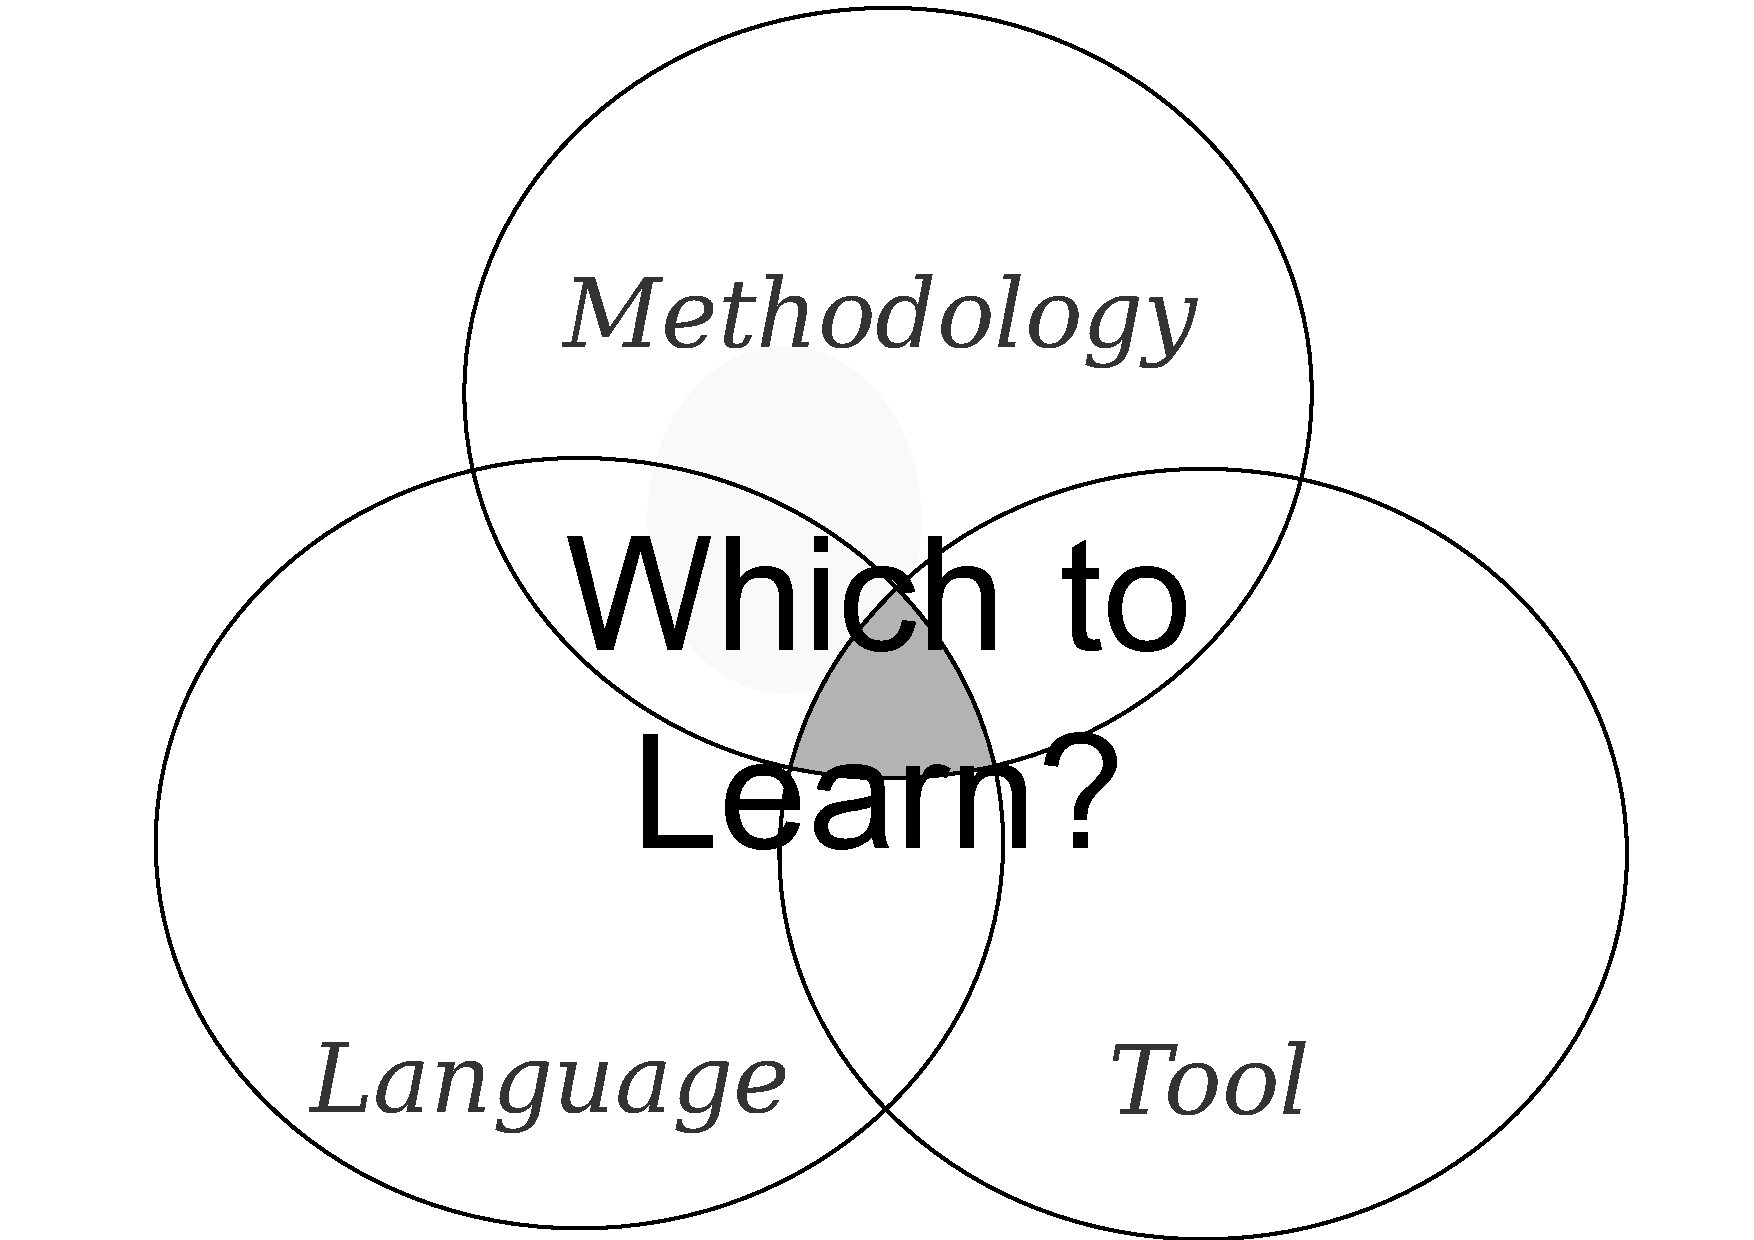
\includegraphics[width=0.6\textwidth]{./figures/FLT_framework.pdf}
\caption{\label{FLT_framework}The Framework-Language-Tool framework.}
\end{figure}
\end{frame}
\begin{frame}[label=sec-1-4-2]{授業で取り上げる範囲}
\begin{block}{取り上げること}
\begin{itemize}
\item 方法を支えるための道具
\item 良い道具には設計概念として方法論が組み込まれている
\item 道具はプログラミング言語を問わない
\end{itemize}
\end{block}
\begin{block}{取り扱わないこと}
\begin{itemize}
\item 方法論そのものについてはアジャイル開発特論で学ぶ
\item 言語の備えるエコシステムについては必要な範囲で学ぶ
\end{itemize}
\end{block}
\end{frame}
\begin{frame}[label=sec-1-4-3]{Scrumするための道具}
\begin{figure}[htb]
\centering
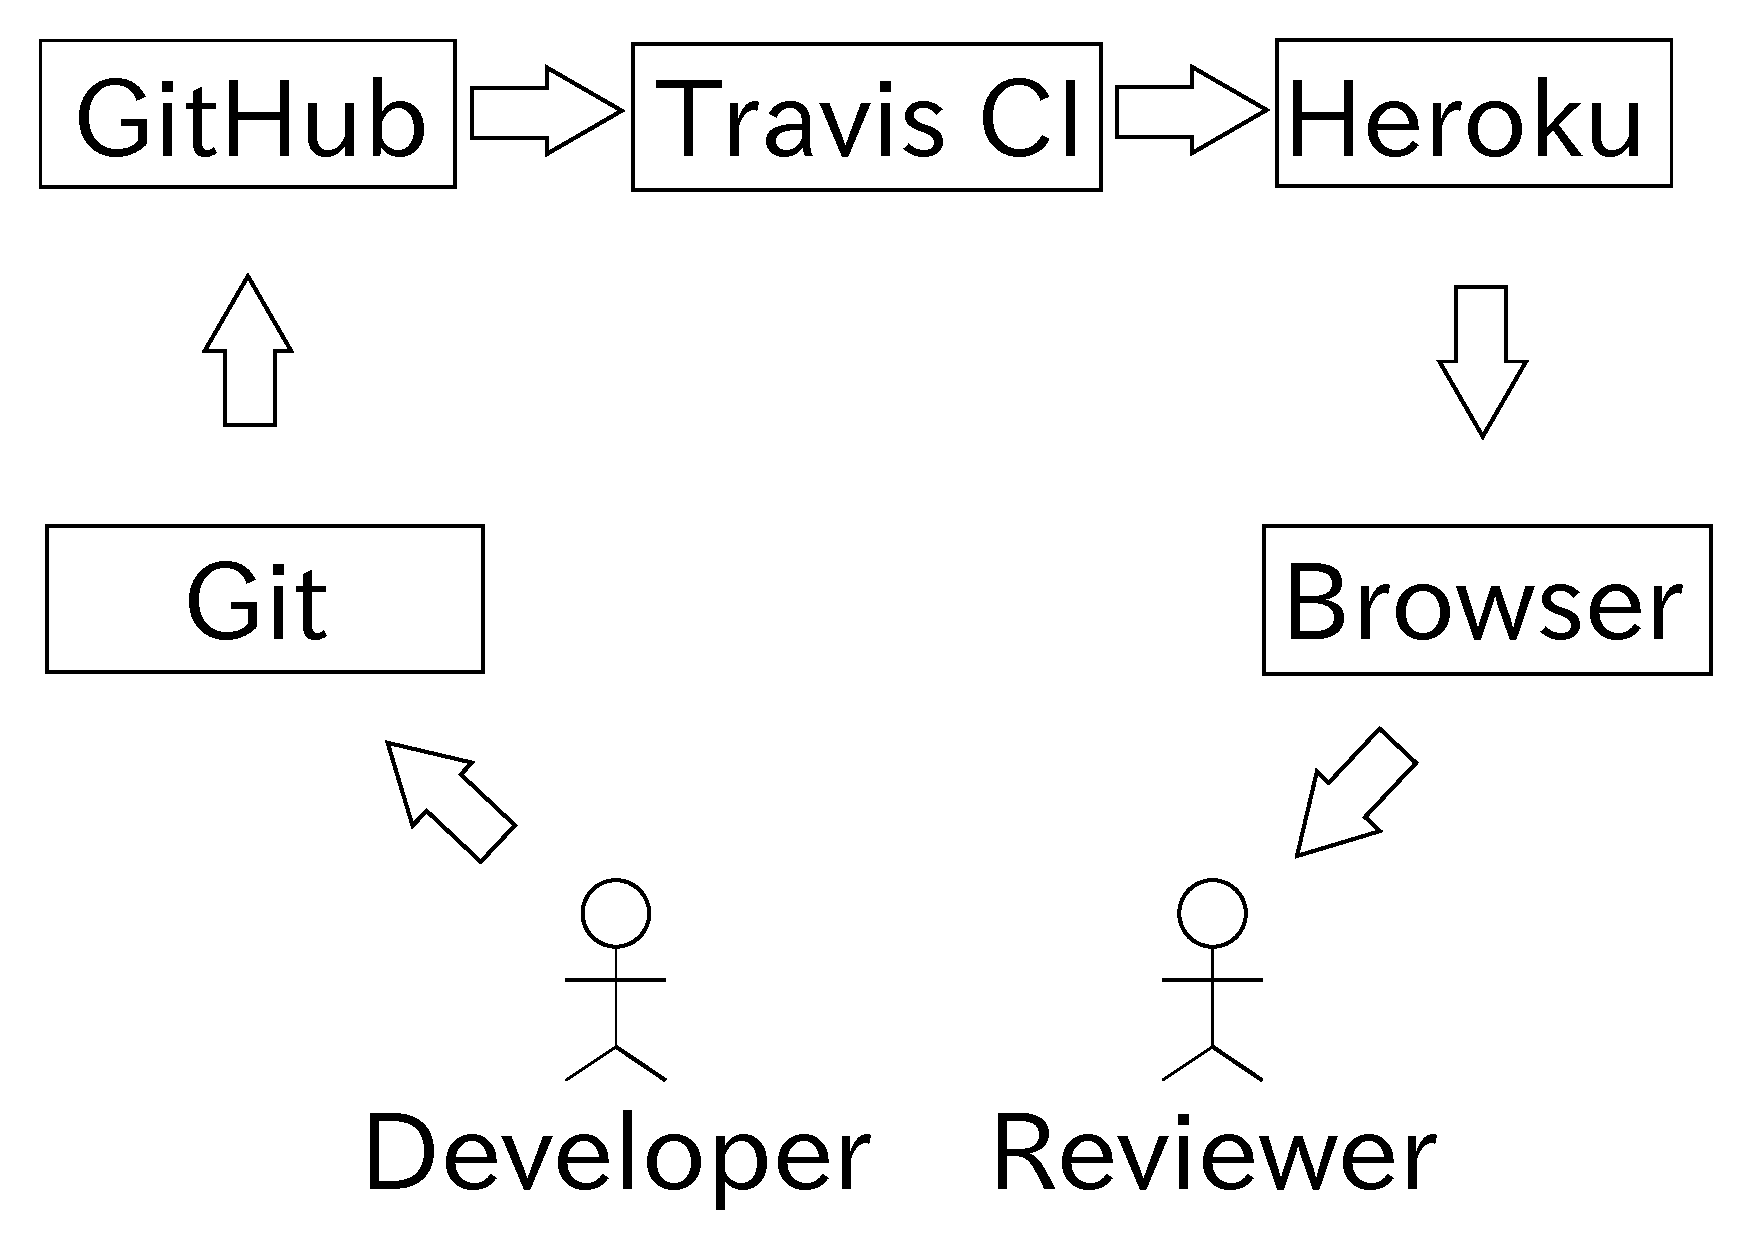
\includegraphics[width=0.6\textwidth]{./figures/tools.pdf}
\caption{\label{tools}The modern tools for Scrum developments.}
\end{figure}
\end{frame}

\begin{frame}[label=sec-1-4-4]{モダンな開発環境の全体像}
\begin{block}{仮想化技術(Virtualization)}
\begin{itemize}
\item WindowsやMacでLinux上でのWebアプリケーション開発を学ぶことができる
\item HerokuやTravis CI等のクラウドでの実行や検査環境として用いられている
\end{itemize}
\end{block}
\begin{block}{ソーシャルコーディング(Social Coding)}
\begin{itemize}
\item LinuxのソースコードのVCSとして用いられているGitを学ぶ
\item GitはGitHubと連携することでOSS型のチーム開発ができる
\end{itemize}
\end{block}
\end{frame}

\begin{frame}[label=sec-1-4-5]{enPiT仮想化環境}
\begin{block}{インストール済みの言語と道具}
\begin{itemize}
\item エディタ(Emacs/Vim)
\item Rubyの実行環境
\item GitHub,Heroku,Travis CIと連携するための各種コマンド(github-connect.sh,hub,heroku,travis)
\item PostgreSQLのクライアント・サーバーとDB
\item 各種設定ファイル(.bash\_profile,.gemrc,.gitconfig)
\item その他
\end{itemize}
\end{block}
\begin{block}{仮想化環境の構築用リポジトリ(参考)}
\begin{itemize}
\item \href{https://github.com/ychubachi/vagrant_enpit}{ychubachi/vagrant\_enpit}
\end{itemize}
\end{block}
\end{frame}
\section{<演習課題(準備作業)>}
\label{sec-1-5}
\begin{frame}[label=sec-1-5-1]{クラウドのアカウント作成}
\begin{block}{GitHub}
\begin{itemize}
\item\relax [\href{https://github.com/join}{Join GitHub · GitHub}]
\end{itemize}
\end{block}
\begin{block}{Heroku}
\begin{itemize}
\item\relax [\href{https://id.heroku.com/signup}{Heroku - Sign up}]
\end{itemize}
\end{block}
\begin{block}{Travis CI}
\begin{itemize}
\item\relax [\href{https://travis-ci.org/}{Travis CI}]
\begin{itemize}
\item Travis CIは,GitHubのアカウントでログインできる
\end{itemize}
\end{itemize}
\end{block}
\end{frame}
\begin{frame}[fragile,label=sec-1-5-2]{enPiT仮想化環境のアップデート}
 \begin{block}{作業内容}
\begin{itemize}
\item enPiT仮想化環境(vagrantのbox)を更新しておく
\end{itemize}
\end{block}
\begin{block}{コマンド}
\begin{minted}[]{bash}
cd ~/enpit
vagrant destroy
vagrant box update
\end{minted}
\end{block}
\end{frame}
\begin{frame}[fragile,label=sec-1-5-3]{Port Forwardの設定}
 \begin{block}{説明}
\begin{itemize}
\item Guest OSで実行するサーバに,Host OSからWebブラウザでアクセスできるようにしておく
\item 任意のエディタでVagrantfileを変更
\end{itemize}
\end{block}
\begin{block}{変更前}
\begin{minted}[]{ruby}
# config.vm.network "forwarded_port", guest: 80, host: 8080
\end{minted}
\end{block}

\begin{block}{変更後}
\begin{minted}[]{ruby}
config.vm.network "forwarded_port", guest: 3000, host: 3000
config.vm.network "forwarded_port", guest: 4567, host: 4567
\end{minted}
\end{block}
\end{frame}

\begin{frame}[fragile,label=sec-1-5-4]{enPiT仮想化環境にログイン}
 \begin{block}{作業内容}
\begin{itemize}
\item 前の操作に引き続き,仮想化環境にSSH接続する
\end{itemize}
\end{block}
\begin{block}{コマンド}
\begin{minted}[]{bash}
vagrant up
vagrant ssh
\end{minted}
\end{block}
\end{frame}

\begin{frame}[label=sec-1-5-5]{github-connectスクリプト}
\begin{block}{URL}
\begin{itemize}
\item\relax [\href{https://gist.github.com/ychubachi/6491682}{github-connect.sh}]
\end{itemize}
\end{block}
\begin{block}{git conifgを代行}
\begin{itemize}
\item GitHubにログインし,名前とemailを読み込んでgitに設定
\end{itemize}
\end{block}
\begin{block}{SSHの鍵生成と登録}
\begin{itemize}
\item SSH鍵を作成し,公開鍵をGitHubに登録してくれる
\end{itemize}
\end{block}
\end{frame}
\begin{frame}[fragile,label=sec-1-5-6]{github-connect.shの実行}
 \begin{block}{作業内容}
\begin{itemize}
\item スクリプトを起動し,設定を行う
\item GitHubのログイン名とパスワードを聞かれるので,入力する
\item rsa key pairのパスフレーズは入力しなくて構わない
\end{itemize}
\end{block}
\begin{block}{コマンド}
\begin{minted}[]{bash}
github-connect.sh
\end{minted}
\end{block}
\end{frame}

\begin{frame}[fragile,label=sec-1-5-7]{GitとGitHubの設定確認}
 \begin{block}{Gitの設定確認}
\begin{minted}[]{bash}
git config --list
\end{minted}
\end{block}
\begin{block}{GitHubの設定確認}
\begin{itemize}
\item ブラウザでGitHubのSSH Keyページを開く
\end{itemize}
\end{block}
\end{frame}

\part{第2章 Git/GitHubの基本操作}
\label{sec-2}
\section{ローカルリポジトリ}
\label{sec-2-1}
\begin{frame}[fragile,label=sec-2-1-1]{Gitのローカルリポジトリの作成}
 \begin{block}{ローカルリポジトリ}
\begin{itemize}
\item ソースコードや各種のファイルを保存し,開発に利用する
\item 「 \texttt{my\_enpit} 」というディレクトリを作成し,初期化する
\end{itemize}
\end{block}
\begin{block}{コマンド}
\begin{minted}[]{bash}
mkdir ~/my_enpit
cd ~/my_enpit
git init
\end{minted}
\end{block}
\end{frame}

\begin{frame}[fragile,label=sec-2-1-2]{Gitの設定ディレクトリ}
 \begin{block}{隠しフォルダ「 \texttt{.git} 」}
\begin{itemize}
\item Gitソースコードの履歴情報や,各種の設定をGitが保存するディレクトリ
\item このフォルダは通常,Gitを経由しないで変更することはない
\end{itemize}
\end{block}
\begin{block}{確認方法}
\begin{minted}[]{bash}
ls -a
find .git
\end{minted}
\end{block}
\end{frame}

\section{リモートリポジトリ}
\label{sec-2-2}
\begin{frame}[fragile,label=sec-2-2-1]{Hubコマンド}
 \begin{block}{enPiT環境のHubコマンド}
\begin{itemize}
\item \href{https://github.com/github/hub}{github/hub}
\end{itemize}
\end{block}
\begin{block}{GitへのGitHub操作機能追加}
\begin{itemize}
\item 通常のGitの機能に加えて,GitHub用のコマンドが利用できる
\item エイリアス設定しており,コマンド名は「git」のまま
\end{itemize}
\end{block}
\begin{block}{確認方法}
\begin{minted}[]{bash}
git version
alias git
\end{minted}
\end{block}
\end{frame}

\begin{frame}[fragile,label=sec-2-2-2]{Hubコマンドによるリモートリポジトリの作成}
 \begin{block}{作業内容}
\begin{itemize}
\item コマンドライン操作で,GitHubにリポジトリを作成する
\item Hubコマンドの機能である \texttt{git create} を利用
\item 初回既動時にはパスワードか聞かれる
\end{itemize}
\end{block}
\begin{block}{コマンド}
\begin{minted}[]{bash}
git create
\end{minted}
\end{block}
\end{frame}

\begin{frame}[fragile,label=sec-2-2-3]{リポジトリの確認方法}
 \begin{block}{確認方法}
\begin{itemize}
\item WebブラウザでGitHubを開き,「 \texttt{my\_enpit} 」ができていることを確認
\end{itemize}
\end{block}
\begin{block}{コマンドラインで確認}
\begin{minted}[]{bash}
git remote -vv
\end{minted}
\end{block}
\end{frame}
\section{GitとGitHubの基本操作}
\label{sec-2-3}
\begin{frame}[label=sec-2-3-1]{Gitの操作方法}
\begin{block}{マニュアル等}
\begin{itemize}
\item \href{http://git-scm.com/doc}{Git - Documentation}
\end{itemize}
\end{block}
\begin{block}{commitログの書き方}
\begin{itemize}
\item \href{https://github.com/erlang/otp/wiki/Writing-good-commit-messages}{Writing good commit messages · erlang/otp Wiki}
\end{itemize}
\end{block}
\end{frame}
\begin{frame}[fragile,label=sec-2-3-2]{ステータスの確認}
 \begin{block}{リポジトリの状態を確認する}
\begin{itemize}
\item \texttt{git status} は,頻繁に利用するコマンド
\item リポジトリの状態を確認することができる
\item この表示の読み方を理解することが重要
\end{itemize}
\end{block}
\begin{block}{コマンド}
\begin{minted}[]{bash}
git status
\end{minted}
\end{block}
\end{frame}

\begin{frame}[fragile,label=sec-2-3-3]{ファイルの追加とステータスの確認}
 \begin{block}{作業内容}
\begin{itemize}
\item テキストエディタで \texttt{README.md} を作成
\item ステータスの変化を見る
\end{itemize}
\end{block}
\begin{block}{コマンド}
\begin{minted}[]{bash}
emacs README.md
git status
\end{minted}
\end{block}
\end{frame}

\begin{frame}[label=sec-2-3-4]{Add/Commitの方法}
\begin{block}{ステージングエリアを利用する場合}
\begin{itemize}
\item git add README.mb
\item git commit -m 'First commit'
\end{itemize}
\end{block}
\begin{block}{ステージングエリアを省略する場合}
\begin{itemize}
\item git commit -a -m 'First commit'
\begin{itemize}
\item トラックされていないファイルはcommitしないので注意
\end{itemize}
\end{itemize}
\end{block}
\end{frame}

\begin{frame}[fragile,label=sec-2-3-5]{リモートリポジトリへの公開}
 \begin{block}{pushとは?}
\begin{itemize}
\item ローカルで作成したcommitを,リモートのリポジトリにアップロードすること
\item originとは,リモートのリポジトリの内部的な名前
\item upstreamとは,ブランチ(後述)が紐づいているリポジトリのこと
\item 最初にそのブランチをpushするときは, \texttt{-{}-setupstream} オプションを指定
\end{itemize}
\end{block}
\begin{block}{コマンド}
\begin{minted}[]{bash}
git push --set-upstream origin master
\end{minted}
\end{block}
\end{frame}

\begin{frame}[fragile,label=sec-2-3-6]{Logの閲覧}
 \begin{block}{コミットログ}
\begin{itemize}
\item ソースコードに加えた変更の履歴を,commitを単位として閲覧できる
\end{itemize}
\end{block}
\begin{block}{コマンド}
\begin{minted}[]{bash}
git log
\end{minted}
\end{block}
\end{frame}

\begin{frame}[fragile,label=sec-2-3-7]{コミットのログを詳細に書く方法}
 \begin{block}{エディタを使ったログの記述}
\begin{itemize}
\item コミットのログや,Pull Requestの記述を,より詳しく書くことができる
\item \texttt{commit} や \texttt{pull\_request} から  \texttt{-m} オプションを外すと,エディタが立ち上がる
\begin{itemize}
\item エディタはemacsを起動するようになっている
\item \texttt{C-x C-s} で保存, \texttt{C-x C-c} で終了
\end{itemize}
\end{itemize}
\end{block}
\begin{block}{コマンド}
\begin{minted}[]{bash}
git commit
git pull_request
\end{minted}
\end{block}
\end{frame}

\section{<演習課題>}
\label{sec-2-4}
\begin{frame}[label=sec-2-4-1]{Init/Status/Addの練習}
\begin{block}{演習課題}
\begin{enumerate}
\item 解説した手順に従い,my\_enpitリポジトリを作成
\item git statusコマンドを実行
\item README.mdファイルを作成しなさい
\item git statusコマンドを実行し,変化を見なさい
\item commitしなさい.ログを必ず書くこと
\item git statusコマンドを実行し,変化を見なさい
\end{enumerate}
\end{block}
\end{frame}
\begin{frame}[fragile,label=sec-2-4-2]{Commit/Log/Pushの練習}
 \begin{block}{演習課題}
\begin{enumerate}
\item README.mdを修正してcommitしなさい
\item 新しいファイルを作成してcommitしなさい
\item 作業が完了したら,pushしなさい( \texttt{-{}-set-upstream} が必要)
\item コミットがpushされていることをWebブラウザで確認しなさい
\item 作成したファイルを削除してcommitしてpushしなさい
\item エディタを使って,詳細なログを書きなさい
\item その他,自由にcommitの作業を試しなさい
\end{enumerate}
\end{block}
\end{frame}
\begin{frame}[label=sec-2-4-3]{ここまでの課題の提出}
\begin{block}{提出物}
\begin{itemize}
\item 下記のものを提出してください
\begin{itemize}
\item GitHubとHerokuアカウント
\item 作成したmy\_enpitリポジトリのURL
\end{itemize}
\end{itemize}
\end{block}
\begin{block}{提出先}
\begin{itemize}
\item\relax [\href{https://docs.google.com/forms/d/1SiKQqDLQw2YiJieYVS79ywpHIaNC3uI9cNPb_ddhC1Q/viewform?usp=send_form}{enPiT演習アカウント(2014)}]
\end{itemize}
\end{block}
\end{frame}

\part{第3章 GitHubを用いた開発の流れ}
\label{sec-3}
\section{GitHub Flow}
\label{sec-3-1}
\begin{frame}[label=sec-3-1-1]{GitHub Flow (1)}
\begin{enumerate}
\item 思い立ったらブランチ作成
\begin{itemize}
\item 新しい機能追加や,アイディアを試す
\end{itemize}
\item ブランチにコミットを追加
\begin{itemize}
\item 変更点をコミットとして作成
\item コミットのログは,他人が読んでわかるように書く
\end{itemize}
\item Pull Requestを開く
\begin{itemize}
\item コミットについて,意見交換ができる
\item 作業途中でPull Requestを出しても構わない
\end{itemize}
\end{enumerate}
\end{frame}
\begin{frame}[fragile,label=sec-3-1-2]{GitHub Flow (2)}
 \begin{enumerate}
\item 議論とレビュー
\begin{itemize}
\item レビューをしたり,質疑応答をしたりする
\end{itemize}
\item マージしてディプロイ
\begin{itemize}
\item \texttt{master} ブランチにマージする(自動でディプロイ)
\item マージの前にテストしたいときは,ローカルで試す
\end{itemize}
\end{enumerate}
参考文献
\begin{itemize}
\item \href{https://guides.github.com/introduction/flow/index.html}{Understanding the GitHub Flow · GitHub Guides}
\end{itemize}
\end{frame}

\section{ブランチの操作}
\label{sec-3-2}
\begin{frame}[fragile,label=sec-3-2-1]{branchの作成}
 \begin{block}{ブランチとは?}
\begin{itemize}
\item リポジトリにはmasterブランチがある
\item 新しい作業を行う場合,必ずbranchを切る
\end{itemize}
\end{block}
\begin{block}{コマンド}
\begin{minted}[]{bash}
git branch new_branch
git branch -vv
\end{minted}
\end{block}
\end{frame}

\begin{frame}[fragile,label=sec-3-2-2]{branchのcheckout}
 \begin{block}{branchを切り替える}
\begin{itemize}
\item checkoutしてブランチを切り替える
\item ブランチをcommitすることができる
\item 切り替える前に,ブランチでの作業はcommitしておく(stashも可)
\end{itemize}
\end{block}
\begin{block}{コマンド}
\begin{minted}[]{bash}
git checkout new_branch
<編集作業>
git commit -a -m 'Create a new branch'
\end{minted}
\end{block}
\end{frame}

\begin{frame}[fragile,label=sec-3-2-3]{他のbranchをmergeする}
 \begin{block}{mergeとは}
\begin{itemize}
\item ブランチで作業した内容(commit)を,他のブランチに統合すること
\item new\_branchでの作業をmasterに統合する場合,最初にmasterをcheckoutする
\end{itemize}
\end{block}
\begin{block}{コマンド操作}
\begin{minted}[]{bash}
git checkout master
git merge new_branch
\end{minted}
\end{block}
\end{frame}

\begin{frame}[label=sec-3-2-4]{Conflict(競合)とその解消}
\begin{block}{Conflictとは}
\begin{itemize}
\item branchで行う作業がかち合った場合,発生する
\item mergeする際,conflictが生じた場合,エラーになる
\end{itemize}
\end{block}
\begin{block}{解消方法}
\begin{itemize}
\item エディタ等で編集を行い,解消する
\end{itemize}
\end{block}
\begin{block}{参考文献}
\begin{itemize}
\item \href{https://help.github.com/articles/resolving-a-merge-conflict-from-the-command-line}{Resolving a merge conflict from the command line · GitHub Help}
\end{itemize}
\end{block}
\end{frame}
\section{リモートのブランチ}
\label{sec-3-3}
\begin{frame}[fragile,label=sec-3-3-1]{BranchのPush}
 \begin{block}{リモートへのPush}
\begin{itemize}
\item BranchをGitHubにPushすることができる
\item masterブランチをPushした際と同様,upstreamを指定する
\item PushできたかどうかをWebブラウザで確認する
\end{itemize}
\end{block}

\begin{block}{コマンド}
\begin{minted}[]{bash}
git push --set-upstream origin new_branch
\end{minted}
\end{block}
\end{frame}

\section{Pull Request}
\label{sec-3-4}
\begin{frame}[fragile,label=sec-3-4-1]{Pull Requestの作成}
 \begin{block}{Pull Roquestとは?}
\begin{itemize}
\item pushしたbranchでの作業の統合(merge)を依頼する
\item hubコマンドの \texttt{pull-request} で発行できる
\end{itemize}
\end{block}

\begin{block}{コマンド}
\begin{minted}[]{bash}
git pull-request -m 'Update a new branch'
\end{minted}
\end{block}
\end{frame}

\begin{frame}[fragile,label=sec-3-4-2]{Pull Requestのmerge}
 \begin{block}{Pull Requestをレビューする}
\begin{itemize}
\item WebブラウザでPull Requestを確認する
\end{itemize}
\end{block}
\begin{block}{ブラウザでmerge}
\begin{itemize}
\item 問題なければmergeボタンを押す
\end{itemize}
\end{block}
\begin{block}{コマンドラインでmergeする場合}
\begin{minted}[]{bash}
git merge pull_request_URL
\end{minted}
\end{block}
\end{frame}

\begin{frame}[fragile,label=sec-3-4-3]{BranchのPull}
 \begin{block}{BranchをPullするとは}
\begin{itemize}
\item リモートで行われた変更を適用すること
\item 内部的にはfetchでダウンロードしてからmergeする
\end{itemize}
\end{block}
\begin{block}{コマンド}
\begin{minted}[]{bash}
git checkout master
git pull
\end{minted}
\end{block}
\end{frame}

\section{<演習課題>}
\label{sec-3-5}
\begin{frame}[fragile,label=sec-3-5-1]{branchの操作(ローカル)}
 \begin{block}{演習課題}
\begin{enumerate}
\item \texttt{my\_enpit} リポジトリでブランチを作成しなさい( \texttt{new\_branch} )
\item \texttt{checkout} で \texttt{new\_branch} に移動する
\item ファイルを編集しcommitする
\item \texttt{master} ブランチに移動してファイルの内容が
「編集されていないこと」を確認しなさい
\item \texttt{merge} して,変更を適用しなさい
\end{enumerate}
\end{block}
\end{frame}
\begin{frame}[fragile,label=sec-3-5-2]{競合の発生と解消}
 \begin{block}{演習課題}
\begin{enumerate}
\item \texttt{new\_branch} でファイルを編集して,commitする
\item \texttt{master} に移動し,ファイルの同じ箇所を編集して,commitする
\item \texttt{master} に \texttt{new\_branch} をmergeして,コンフリクトを発生させる
\item エディタで競合箇所を修正してcommitする
\end{enumerate}
\end{block}
\end{frame}
\begin{frame}[fragile,label=sec-3-5-3]{リモートのbranchの操作}
 \begin{block}{演習課題}
\begin{enumerate}
\item 新しいブランチを作成して,remoteにpushする
\item Pull Requestを送る
\item ブラウザで,Pull Requestをマージする
\item \texttt{master} ブランチに移動して, \texttt{pull} することで,更新する
\end{enumerate}
\end{block}
\end{frame}
\part{第4章 GitHubによる協同作業}
\label{sec-4}
\section{他の人の開発状況を見る}
\label{sec-4-1}
\begin{frame}[fragile,label=sec-4-1-1]{リモートのリポジトリをClone}
 \begin{block}{Cloneとは}
\begin{itemize}
\item GitHubで公開されているリポジトリはだれでも複製(clone)できる
\item ソースコードはローカルにコピーされ,閲覧やコンパイルなどができるようになる
\item アクセス権限がない場合は,pushできない
\end{itemize}
\end{block}
\begin{block}{コマンド}
\begin{minted}[]{bash}
git clone octocat/Spoon-Knife
\end{minted}
\end{block}
\end{frame}

\begin{frame}[fragile,label=sec-4-1-2]{Pull Requestをチェックアウト}
 \begin{block}{Pull Requestのチェックアウト}
\begin{itemize}
\item 誰かが作成したPull Requestの内容を,ブランチとしてローカルにコピーする
\item 試しに動作させたり,コードをチェックするときなどに利用
\end{itemize}
\end{block}
\begin{block}{コマンド}
\begin{minted}[]{bash}
git checkout https://github.com/octocat/Spoon-Knife/pull/3166
\end{minted}
\end{block}
\end{frame}

\section{開発に参加する}
\label{sec-4-2}
\begin{frame}[fragile,label=sec-4-2-1]{オリジナルのリポジトリをForkする}
 \begin{block}{Forkとは}
\begin{itemize}
\item Cloneしたリポジトリを,
自分のアカウントが所持するリポジトリとして
GitHub上で複製する
\item \texttt{remote} の値は,オリジナルのリポジトリが \texttt{origin} ,
自分のリポジトリは自分のGitHubユーザ名になる
\end{itemize}
\end{block}
\begin{block}{コマンド}
\begin{minted}[]{bash}
git fork
git remote -vv
\end{minted}
\end{block}
\end{frame}

\begin{frame}[fragile,label=sec-4-2-2]{ブランチを作成し自分のリポジトリにpush}
 \begin{block}{オリジナルの改変等}
\begin{itemize}
\item 新しい機能追加等を行う場合,ブランチを作成する
\item ブランチは,自分のリポジトリにpushする
\end{itemize}
\end{block}
\begin{block}{コマンド}
\begin{minted}[]{bash}
git branch my_branch
git checkout my_branch
<編集>
git commit -a -m 'Update'
git push -u ychubachi my_branch
\end{minted}
\end{block}
\end{frame}

\begin{frame}[fragile,label=sec-4-2-3]{Forkした元にPull Requestを送る}
 \begin{block}{コードのレビューやマージを依頼する}
\begin{itemize}
\item 新しい機能ができたら,オリジナルにPull Requestを送り,
レビューやマージをしてもらう
\end{itemize}
\end{block}
\begin{block}{コマンド}
\begin{minted}[]{bash}
git pull_request -m 'Pull Request'
\end{minted}
\end{block}
\end{frame}

\section{GitHubの他の機能}
\label{sec-4-3}
\begin{frame}[label=sec-4-3-1]{Issue/Wiki}
\begin{block}{Issue}
\begin{itemize}
\item 課題管理(ITS: Issue Tracking System)
\item コミットのメッセージでcloseできる
\begin{itemize}
\item \href{https://help.github.com/articles/closing-issues-via-commit-messages}{Closing issues via commit messages · GitHub Help}
\end{itemize}
\end{itemize}
\end{block}
\begin{block}{Wiki}
\begin{itemize}
\item GitHubのリポジトリにWikiを作る
\begin{itemize}
\item \href{https://help.github.com/articles/about-github-wikis}{About GitHub Wikis · GitHub Help}
\end{itemize}
\end{itemize}
\end{block}
\end{frame}
\begin{frame}[label=sec-4-3-2]{GitHub}
\begin{block}{GitHub Pages}
\begin{itemize}
\item 特殊なブランチを作成すると,Webページが構築できる
\begin{itemize}
\item \href{https://pages.github.com/}{GitHub Pages}
\end{itemize}
\end{itemize}
\end{block}
\begin{block}{Git brame}
\begin{itemize}
\item だれがどの作業をしたかわかる(誰がバグを仕込んだのかも)
\begin{itemize}
\item \href{https://help.github.com/articles/using-git-blame-to-trace-changes-in-a-file}{Using git blame to trace changes in a file · GitHub Help}
\end{itemize}
\end{itemize}
\end{block}
\end{frame}
\section{<演習課題>}
\label{sec-4-4}
\begin{frame}[fragile,label=sec-4-4-1]{our\_enpitにファイルを追加する}
 \begin{block}{演習課題}
\begin{enumerate}
\item \texttt{ychubich/our\_enpit} をcloneしてforkする
\item 新しいブランチを作成し,新規にファイルを追加する
\begin{itemize}
\item 内容は任意(自己紹介など)
\item Markdownで書いてください(拡張子は.md)
\end{itemize}
\item コミットを作成し,pull requestを送信する
\item 教員がマージ作業を行います
\end{enumerate}
\end{block}
\end{frame}
\begin{frame}[label=sec-4-4-2]{既存のファイルを変更する}
\begin{block}{演習課題}
\begin{enumerate}
\item README.mdを改変して,pull requestを送信する
\item GitHubのPull Request一覧を確認する
\item おそらくコンフリクトが発生するので,
GitHubの指示に従い競合を解消する
\end{enumerate}
\end{block}
\end{frame}
\begin{frame}[label=sec-4-4-3]{隣の人との協同作業}
\begin{block}{演習課題}
\begin{enumerate}
\item 新しくリポジトリを作成する(名称は任意)
\item 互いに,隣の席の人にリポジトリ名を教え,forkしてもらい
Pull Requestを送ってもらう
\item マージしてあげる
\item 2〜3を繰り返し,協同作業を行ってみよう
\end{enumerate}
\end{block}
\end{frame}
\begin{frame}[label=sec-4-4-4]{Issue/Wikiの利用}
\begin{block}{演習課題}
\begin{itemize}
\item GitHubのIssueの機能を使ってみなさい
\item commitのログでIssueをクローズさせてみなさい
\item Wikiを作ってください
\end{itemize}
\end{block}
\end{frame}
\part{第5章 Sinatraアプリの開発}
\label{sec-5}
\section{Sinatraアプリケーションの作成}
\label{sec-5-1}
\begin{frame}[label=sec-5-1-1]{Sinatraを使った簡単なWebアプリケーション}
\begin{block}{Sinatraとは?}
\begin{itemize}
\item Webアプリケーションを作成するDSL
\item Railsに比べ軽量で,学習曲線が緩やか
\end{itemize}
\end{block}
\begin{block}{参考文献}
\begin{itemize}
\item \href{http://www.sinatrarb.com/}{Sinatra}
\end{itemize}
\end{block}
\end{frame}

\begin{frame}[fragile,label=sec-5-1-2]{Sinatraアプリ用リポジトリを作成する}
 \begin{block}{内容}
\begin{itemize}
\item Sinatraアプリを作成するため,新しいリポジトリを作る
\end{itemize}
\end{block}
\begin{block}{コマンド}
\begin{minted}[]{bash}
mkdir ~/sinatra_enpit
cd ~/shinatra_enpit
git init
git create
\end{minted}
\end{block}
\end{frame}

\begin{frame}[fragile,label=sec-5-1-3]{Sinatraアプリを作成する}
 \begin{block}{コマンド}
\begin{minted}[]{bash}
emacs hello.rb
git add hello.rb
git commit -m 'Create hello.rb'
\end{minted}
\end{block}

\begin{block}{コード: \texttt{hello.rb}}
\begin{minted}[]{ruby}
require 'sinatra'

get '/' do
  "Hello World!"
end
\end{minted}
\end{block}
\end{frame}

\begin{frame}[fragile,label=sec-5-1-4]{Sinatraアプリを起動する}
 \begin{block}{起動の方法}
\begin{itemize}
\item hello.rbをrubyで動かせば,サーバが立ち上がる
\item vagrantのport forwardを利用するためのオプションを追加する
\begin{itemize}
\item \href{http://stackoverflow.com/questions/21250885/unable-to-access-sinatra-app-on-host-machine-with-vagrant-forwarded-ports}{ruby - Unable to access Sinatra app on host machine with Vagrant forwarded ports - Stack Overflow}
\end{itemize}
\end{itemize}
\end{block}

\begin{block}{コマンド}
\begin{minted}[]{bash}
ruby hello.rb -o 0.0.0.0
\end{minted}
\end{block}
\end{frame}

\begin{frame}[label=sec-5-1-5]{Sinatraアプリの動作確認}
\begin{block}{動作確認の方法}
\begin{itemize}
\item Host OSのWebブラウザで,\url{http://localhost:4567} にアクセスする.
\end{itemize}
\end{block}
\end{frame}

\section{Herokuでアプリケーションを動かす}
\label{sec-5-2}
\begin{frame}[fragile,label=sec-5-2-1]{コマンドラインでHerokuにログインする}
 \begin{block}{内容}
\begin{itemize}
\item enPiT環境には \texttt{heroku} コマンドをインストールしてある
\item \texttt{heroku} コマンドを用いて,Herokuにログインできる
\item 以後の作業はHerokuコマンドを利用する
\end{itemize}
\end{block}
\begin{block}{コマンド}
\begin{minted}[]{bash}
heroku login
\end{minted}
\end{block}
\end{frame}

\begin{frame}[fragile,label=sec-5-2-2]{herokuにSSHの公開鍵を設定する}
 \begin{block}{内容}
\begin{itemize}
\item Herokuもgitのリモートリポジトリである
\item ここに公開鍵でアクセスできるようにする
\end{itemize}
\end{block}
\begin{block}{コマンド}
\begin{minted}[]{bash}
heroku keys:add
\end{minted}
\end{block}
\begin{block}{確認}
\begin{minted}[]{bash}
heroku keys
\end{minted}
\end{block}
\end{frame}

\begin{frame}[fragile,label=sec-5-2-3]{Herokuで動作できるSinatraアプリ}
 \begin{block}{内容}
\begin{itemize}
\item Herokuで動作できるSinatraアプリと設定ファイルの例
\href{https://devcenter.heroku.com/articles/rack#sinatra}{Deploying Rack-based Apps | Heroku Dev Center}
\item 例を見ながら,エディタを用いて,次の3つのファイルを作成する
\begin{description}
\item[{\texttt{hello.rb}}] RubyによるWebアプリ本体(作成済み)
\item[{\texttt{config.ru}}] Webアプリサーバ(Rack)の設定
\item[{\texttt{Gemfile}}] アプリで利用するライブラリ(Gem)
\end{description}
\end{itemize}
\end{block}
\begin{block}{コマンド}
\begin{minted}[]{bash}
emacs config.ru
emacs Gemfile
\end{minted}
\end{block}
\end{frame}

\begin{frame}[fragile,label=sec-5-2-4]{アプリをGitHubにpushする}
 \begin{block}{内容}
\begin{itemize}
\item Herokuで動かす前に,commitが必要
\item ついでに,GitHubにコードをpushしておく
\begin{itemize}
\item この場合のpush先は \texttt{origin master}
\end{itemize}
\end{itemize}
\end{block}
\begin{block}{コマンド}
\begin{minted}[]{bash}
git add .
git commit -m 'Add configuration files for Heroku'
git push origin master
\end{minted}
\end{block}
\end{frame}

\begin{frame}[fragile,label=sec-5-2-5]{Herokuにアプリを作る}
 \begin{block}{アプリを作る}
\begin{itemize}
\item Herokuが自動生成したURLが表示されるので,メモする
\item \texttt{git remote -v} でherokuという名前のremoteが追加されたことが分かる
\item WebブラウザでHerokuの管理画面を開くと,アプリができていることが確認できる
\end{itemize}
\end{block}

\begin{block}{コマンド}
\begin{minted}[]{bash}
heroku create
git remote -v
\end{minted}
\end{block}
\end{frame}

\begin{frame}[fragile,label=sec-5-2-6]{Herokuにアプリを配備する}
 \begin{block}{配備する方法}
\begin{itemize}
\item Herokuのリモートリポジトリにpushする
\item WebブラウザでアプリのURLを開き,動作を確認する
\end{itemize}
\end{block}
\begin{block}{コマンド}
\begin{minted}[]{bash}
git push heroku master
\end{minted}
\end{block}
\end{frame}

\section{<演習課題>}
\label{sec-5-3}
\begin{frame}[label=sec-5-3-1]{Sinatraアプリの作成}
\begin{block}{演習課題}
\begin{itemize}
\item Sinatraアプリを作成して,Herokuで動作させなさい
\item SinatraのDSLについて調べ,機能を追加しなさい
\item コミットのログは詳細に記述し,どんな作業を行ったかが
他の人にも分かるようにしなさい
\item 完成したコードはGitHubにもpushしなさい
\end{itemize}
\end{block}
\end{frame}
\begin{frame}[label=sec-5-3-2]{Sinatraアプリの共同開発}
\begin{block}{演習課題}
\begin{itemize}
\item 隣の席の人と協同でSinatraアプリを開発しなさい
\item 一方がGitHubのリポジトリを作成し,もう一人がForkする
\item 最初に,どんな機能をもたせるかを相談しなさい
\begin{itemize}
\item メンバーのスキルに合わせて,できるだけ簡単なもの
\item データベースは使わない
\end{itemize}
\item ブランチを作成し,Pull Requestを送る
\end{itemize}
\end{block}
\end{frame}

\part{第6章 Ruby on Railsアプリの開発}
\label{sec-6}
\section{Ruby on Railsアプリの生成と実行}
\label{sec-6-1}
\begin{frame}[label=sec-6-1-1]{RoRを使ったWebアプリケーション}
\begin{block}{Ruby on Rails(RoR)とは?}
\begin{itemize}
\item Webアプリケーションを作成するためのフレームワーク
\end{itemize}
\end{block}
\begin{block}{参考文献}
\begin{itemize}
\item \href{http://rubyonrails.org/}{Ruby on Rails}
\end{itemize}
\end{block}
\end{frame}

\begin{frame}[label=sec-6-1-2]{Herokuで動かす方法}
\begin{block}{Getting Started}
\begin{itemize}
\item \href{https://devcenter.heroku.com/articles/getting-started-with-rails4}{Getting Started with Rails 4.x on Heroku | Heroku Dev Center}
\end{itemize}
\end{block}

\begin{block}{DBについて}
\begin{itemize}
\item DatabeseはPostgreSQLを使用する
\begin{itemize}
\item RoR標準のsqliteは使わない
\end{itemize}
\end{itemize}
\end{block}
\end{frame}
\begin{frame}[fragile,label=sec-6-1-3]{\texttt{rails\_enpit} リポジトリを作成する}
 \begin{block}{内容}
\begin{itemize}
\item \texttt{rails} は予め,仮想化環境にインストールしてある
\item \texttt{rails new} コマンドを用いて,RoRアプリの雛形を作成する
\end{itemize}
\end{block}
\begin{block}{コマンド}
\begin{minted}[]{bash}
rails new ~/rails_enpit --database=postgresql
cd ~/rails_enpit
git init
git create
git add .
git commit -m 'Generate a new rails app'
git push -u origin master
\end{minted}
\end{block}
\end{frame}

\begin{frame}[fragile,label=sec-6-1-4]{Gemfileの変更}
 \begin{block}{変更する内容}
\begin{itemize}
\item GemfileにRails内部で動作するJavaScriptの実行環境を設定する
\item 当該箇所のコメントを外す
\item 変更をcommitしておく
\end{itemize}
\end{block}
\begin{block}{変更前}
\begin{minted}[]{ruby}
# gem 'therubyracer',  platforms: :ruby
\end{minted}
\end{block}

\begin{block}{変更後}
\begin{minted}[]{ruby}
gem 'therubyracer',  platforms: :ruby
\end{minted}
\end{block}
\end{frame}

\begin{frame}[fragile,label=sec-6-1-5]{Bundle installの実行}
 \begin{block}{\texttt{bundle install}}
\begin{itemize}
\item Gemfileを読み込み,必要なgemをインストールする
\item \texttt{rails new} をした際にも, \texttt{bundle install} は実行されている
\item 今回はtherubyracerと,それが依存しているgemでまだインストールしていないものをインストール
\item インストールする先は \texttt{\textasciitilde{}/.rbenv} 以下の特定のディレクトリ
\end{itemize}
\end{block}
\begin{block}{コマンド}
\begin{minted}[]{bash}
bundle install
git commit -a -m 'Run bundle install'
\end{minted}
\end{block}
\end{frame}

\begin{frame}[fragile,label=sec-6-1-6]{Rails serverの起動}
 \begin{block}{Rails serverを起動}
\begin{itemize}
\item この段階で,アプリケーションを起動できるようになっている
\item Host OSのWebブラウザで, \texttt{http://localhost:3000} にアクセスして確認
\item 端末にもログが表示される
\item 確認したら,端末でCtrl-Cを押してサーバを停止する
\end{itemize}
\end{block}
\begin{block}{コマンド}
\begin{minted}[]{bash}
rails server
\end{minted}
\end{block}
\end{frame}

\section{Controller/Viewの作成}
\label{sec-6-2}
\begin{frame}[fragile,label=sec-6-2-1]{Hello Worldを表示するController}
 \begin{block}{Controllerとは?}
\begin{itemize}
\item MVC構造でいうController
\item HTTPのリクエストを処理し,Viewに引き渡す
\item \texttt{rails generate controller} コマンドで作成する
\end{itemize}
\end{block}
\begin{block}{コマンド}
\begin{minted}[]{bash}
rails generate controller welcome
\end{minted}
\end{block}
\end{frame}
\begin{frame}[fragile,label=sec-6-2-2]{Viewの作成}
 \begin{block}{Viewとは?}
\begin{itemize}
\item HTML等で結果をレンダリングして表示する
\item \texttt{app/views/welcome/inde.html.erb} を作成する
\item erbで作成するのが一般的で,内部でRubyコードを動作させることができる
\end{itemize}
\end{block}
\begin{block}{\texttt{index.html.erb}}
\begin{minted}[]{html}
<h2>Hello World</h2>
<p>
  The time is now: <%= Time.now %>
</p>
\end{minted}
\end{block}
\end{frame}

\begin{frame}[fragile,label=sec-6-2-3]{rootとなるrouteの設定}
 \begin{block}{Routeとは?}
\begin{itemize}
\item HTTPのリクエスト(URL)とコントローラを紐付ける設定
\item ここでは \texttt{root} へのリクエスト( \texttt{GET /} )を \texttt{welcome} コントローラの \texttt{index} メソッドに紐付ける
\item \texttt{rake routes} で確認する
\end{itemize}
\end{block}
\begin{block}{\texttt{config/routes.rb} の当該箇所をアンコメント}
\begin{minted}[]{ruby}
root 'welcome#index'
\end{minted}
\end{block}
\end{frame}

\begin{frame}[fragile,label=sec-6-2-4]{ControllerとViewの動作確認}
 \begin{block}{動作確認の方法}
\begin{itemize}
\item 再度, \texttt{rails server} でアプリを起動する
\item Webブラウザで \texttt{http://localhost:3000/} を開いて確認する
\end{itemize}
\end{block}
\begin{block}{コマンド}
\begin{minted}[]{bash}
rails server
\end{minted}
\end{block}
\end{frame}

\begin{frame}[fragile,label=sec-6-2-5]{ここまでをコミットしておく}
 \begin{block}{ここまでの内容}
\begin{itemize}
\item ここまでの作業で,controllerとviewを1つ備えるRoRアプリができた
\item 作業が一区切りしたので,commitする
(commitはひとかたまりの作業に対して行う)
\end{itemize}
\end{block}
\begin{block}{コマンド}
\begin{minted}[]{bash}
git add .
git commit -m 'Create welcome controller and view'
\end{minted}
\end{block}
\end{frame}

\section{Herokuにディプロイする}
\label{sec-6-3}
\begin{frame}[fragile,label=sec-6-3-1]{Gemfileの設定}
 \begin{block}{Heroku用Gem}
\begin{itemize}
\item \texttt{Gemfile} に \texttt{rails\_12factor} を追加する
\item Rubyのバージョンも指定しておく
\item \texttt{Gemfile} を変更したら必ず \texttt{bundle install} すること
\end{itemize}
\end{block}

\begin{block}{\texttt{Gemfile} に追加する内容}
\begin{minted}[]{ruby}
gem 'rails_12factor', group: :production
ruby '2.1.2'
\end{minted}
\end{block}
\end{frame}

\begin{frame}[fragile,label=sec-6-3-2]{Gitにコミット}
 \begin{block}{コミットする必要性}
\begin{itemize}
\item Herokuにコードを送るには,gitを用いる
\item ローカルで最新版をcommitしておく必要がある
\item ついでにGitHubにもpushしておく
\end{itemize}
\end{block}
\begin{block}{コマンド}
\begin{minted}[]{bash}
git commit -a -m 'Set up for Heroku'
git push # origin master -> GitHub が省略されている
\end{minted}
\end{block}
\end{frame}

\begin{frame}[fragile,label=sec-6-3-3]{Herokuアプリの作成とディプロイ}
 \begin{block}{作成とディプロイ}
\begin{itemize}
\item \texttt{heroku} コマンドを利用してアプリを作成する
\item \texttt{heroku create} で表示されたURLを開く
\item \texttt{git push} でディプロイすると,Herokuからのログが流れてくる
\end{itemize}
\end{block}
\begin{block}{コマンド}
\begin{minted}[]{bash}
heroku create
git push heroku master
\end{minted}
\end{block}
\end{frame}

\section{<演習課題>}
\label{sec-6-4}
\begin{frame}[label=sec-6-4-1]{RoRアプリの作成}
\begin{block}{演習課題}
\begin{itemize}
\item ここまでの説明に従い,Herokuで動作するRoRアプリを完成させなさい
\end{itemize}
\end{block}
\end{frame}

\part{第7章 DBを使うアプリの開発と継続的統合}
\label{sec-7}
\section{DBとScaffoldの作成}
\label{sec-7-1}
\begin{frame}[fragile,label=sec-7-1-1]{PostgreSQLにDBを作成}
 \begin{block}{開発で利用するDB}
\begin{description}
\item[{rails\_enpit\_development}] 開発作業中に利用
\item[{rails\_enpit\_test}] テスト用に利用
\item[{rails\_enpit\_production}] 本番環境で利用(ローカルには作成しない)
\end{description}
\end{block}
\begin{block}{コマンド}
\begin{minted}[]{bash}
createdb rails_enpit_development
createdb rails_enpit_test
\end{minted}
\end{block}
\end{frame}

\begin{frame}[fragile,label=sec-7-1-2]{Scaffold}
 \begin{block}{Scaffoldとは}
\begin{itemize}
\item \href{https://www.google.co.jp/search?q=scaffold&client=ubuntu&hs=PiK&channel=fs&hl=ja&source=lnms&tbm=isch&sa=X&ei=smUdVKaZKY7s8AXew4LwDw&ved=0CAgQ_AUoAQ&biw=1195&bih=925}{scaffold - Google 検索}
\item RoRでは,MVCの雛形を作る
\begin{itemize}
\item CRUD処理が全て実装される
\end{itemize}
\item 多くのコードが自動生成されるので,branchを切っておくと良い
\begin{itemize}
\item 動作が確認できたらbranchをマージ
\item うまく行かなかったらbranchごと削除すれば良い
\end{itemize}
\end{itemize}
\end{block}
\begin{block}{コマンド}
\begin{minted}[]{bash}
git branch books
git checkout books
rails generate scaffold book title:string author:string
\end{minted}
\end{block}
\end{frame}

\begin{frame}[fragile,label=sec-7-1-3]{DBのmigrate}
 \begin{block}{migrateとは}
\begin{itemize}
\item Databaseのスキーマ定義の更新
\item Scaffoldを追加したり,属性を追加したりした際に行う
\end{itemize}
\end{block}
\begin{block}{コマンド}
\begin{minted}[]{bash}
rake db:migrate
\end{minted}
\end{block}
\end{frame}

\begin{frame}[fragile,label=sec-7-1-4]{routeの確認}
 \begin{block}{route}
\begin{itemize}
\item ルーティングの設定を確認しよう
\end{itemize}
\end{block}
\begin{block}{コマンド}
\begin{minted}[]{bash}
rake routes
\end{minted}
\end{block}
\end{frame}

\begin{frame}[fragile,label=sec-7-1-5]{動作確認}
 \begin{block}{動作確認の方法}
\begin{itemize}
\item Webブラウザで \url{http://localhost:3000/books} を開く
\item CRUD処理が完成していることを確かめる
\end{itemize}
\end{block}
\begin{block}{コマンド}
\begin{minted}[]{bash}
rails server
\end{minted}
\end{block}
\end{frame}

\begin{frame}[fragile,label=sec-7-1-6]{完成したコードをマージ}
 \begin{block}{ブランチをマージ}
\begin{itemize}
\item 動作確認できたので, \texttt{books} branchをマージする
\item 不要になったブランチは, \texttt{git branch -d} で削除する
\end{itemize}
\end{block}
\begin{block}{コマンド}
\begin{minted}[]{bash}
git add .
git commit -m 'Generate books scaffold'
git checkout master
git merge books
git branch -d books
\end{minted}
\end{block}
\end{frame}

\begin{frame}[fragile,label=sec-7-1-7]{Herokuにディプロイ}
 \begin{block}{ディプロイ}
\begin{itemize}
\item ここまでのアプリをディプロイする
\item herokuにあるdbもmigrateする
\item Webブラウザで動作確認する
\end{itemize}
\end{block}
\begin{block}{コマンド}
\begin{minted}[]{bash}
git push heroku master
heroku run db:migrate
\end{minted}
\end{block}
\end{frame}

\begin{frame}[fragile,label=sec-7-1-8]{Scaffoldの作成を取り消す場合(参考)}
 \begin{block}{取り消す操作}
\begin{itemize}
\item migrationを取り消す
\item branchに一旦コミットして,masterブランチに移動
\item branchを削除
\end{itemize}
\end{block}
\begin{block}{コマンド}
\begin{minted}[]{bash}
rake db:rollback
git add .
git commit -m 'Rollback'
git checkout master
git branch -D books
\end{minted}
\end{block}
\end{frame}

\begin{frame}[label=sec-7-1-9]{PostgereSQLクライアントのコマンド(参考)}
\begin{itemize}
\item psqlでDBにログイン
\end{itemize}

\begin{center}
\begin{tabular}{ll}
Backslashコマンド & 説明\\
\hline
l & DBの一覧\\
c & DBに接続\\
d & リレーションの一覧\\
q & 終了\\
\end{tabular}
\end{center}
\end{frame}
\section{RoRアプリのテスト}
\label{sec-7-2}
\begin{frame}[label=sec-7-2-1]{テストについて}
\begin{block}{ガイド}
\begin{itemize}
\item \href{http://guides.rubyonrails.org/testing.html}{A Guide to Testing Rails Applications — Ruby on Rails Guides}
\end{itemize}
\end{block}
\end{frame}

\begin{frame}[fragile,label=sec-7-2-2]{テストの実行}
 \begin{block}{テストコード}
\begin{itemize}
\item Scaffoldはテストコードも作成してくれる
\item テスト用のDB( \texttt{rails\_enpit\_test} )が更新される
\end{itemize}
\end{block}
\begin{block}{コマンド}
\begin{minted}[]{bash}
rake test
\end{minted}
\end{block}
\end{frame}

\section{Travis CIとの連携}
\label{sec-7-3}
\begin{frame}[label=sec-7-3-1]{Travis CI}
− \href{http://docs.travis-ci.com/user/languages/ruby/}{Travis CI: Building a Ruby Project}
\end{frame}

\begin{frame}[fragile,label=sec-7-3-2]{Travisの初期化}
 \begin{block}{内容}
\begin{itemize}
\item Travisにログインして初期化を行う
\item 作業の前にブランチを切る
\item \texttt{init} すると \texttt{.travis.yml} ができる
\end{itemize}
\end{block}
\begin{block}{コマンド}
\begin{minted}[]{bash}
git checkout -b travis # -b -> ブランチを作成
travis login --auto    # GitHubのログイン情報でログイン
travis init            # 質問には全てEnterを押す
\end{minted}
\end{block}
\end{frame}

\begin{frame}[fragile,label=sec-7-3-3]{Herokuとの連携}
 \begin{block}{Herokuとの連携}
\begin{itemize}
\item Travis CIからHerokuへの接続を設定する
\item master以外のブランチで実行すると,そのブランチのみHerokuに送る(ようだ)
\begin{itemize}
\item \href{http://docs.travis-ci.com/user/deployment/heroku/}{Travis CI: Heroku Deployment}
\end{itemize}
\end{itemize}
\end{block}
\begin{block}{コマンド}
\begin{minted}[]{bash}
travis setup heroku
\end{minted}
\end{block}
\end{frame}

\begin{frame}[fragile,label=sec-7-3-4]{Travisで動かすRubyのバージョン設定}
 \begin{block}{設定ファイルの変更}
\begin{itemize}
\item Rubyのバージョン
\end{itemize}
\end{block}
\begin{block}{.travis.yml(抜粋)}
\begin{minted}[]{yaml}
language: ruby
rvm:
- 2.1.2
\end{minted}
\end{block}
\end{frame}

\begin{frame}[fragile,label=sec-7-3-5]{Travis用DB設定ファイル}
 \begin{block}{TravisでのテストDB}
− テストDB用の設定ファイルを追加する
\end{block}
\begin{block}{\texttt{config/database.yml.travis}}
\begin{minted}[]{yaml}
test:
  adapter: postgresql
  database: travis_ci_test
  username: postgres
\end{minted}
\end{block}
\end{frame}

\begin{frame}[fragile,label=sec-7-3-6]{Travis上のDB設定}
 \begin{block}{設定ファイルの変更(追加)}
\begin{itemize}
\item PostgreSQLのバージョン
\item DBの作成
\item \href{http://docs.travis-ci.com/user/using-postgresql/}{Travis CI: Using PostgreSQl on Travis CI}
\end{itemize}
\end{block}

\begin{block}{.travis.yml(抜粋)}
\begin{minted}[]{yaml}
addons:
  postgresql: "9.3"
before_script:
  - psql -c 'create database travis_ci_test;' -U postgres
  - cp config/database.yml.travis config/database.yml
\end{minted}
\end{block}
\end{frame}

\begin{frame}[fragile,label=sec-7-3-7]{GitHubとTravis CI連携}
 \begin{block}{説明}
\begin{itemize}
\item ここまでの設定で,GitHubにpushされたコードは,
Travis CIでテストされ,テストが通ったコミットが
Herokuに送られるようになった
\item WebブラウザでTravis CIを開いて確認する
\end{itemize}
\end{block}
\begin{block}{コマンド}
\begin{minted}[]{bash}
git add .
git commit -m 'Configure Travis CI'
git push
\end{minted}
\end{block}
\end{frame}

\begin{frame}[label=sec-7-3-8]{Travis経由でのHerokuへのdeploy}
\begin{block}{Travisのログを閲覧}
\begin{itemize}
\item WebブラウザでTravis CIの画面を開く
\item ログを読む
\end{itemize}
\end{block}
\begin{block}{HerokuへのDeploy}
\begin{itemize}
\item テストが通れば,自動でHerokuに配備される
\item 配備できたらWebブラウザでアプリのページを開いて確認する
\end{itemize}
\end{block}
\end{frame}
\section{<演習課題>}
\label{sec-7-4}
\begin{frame}[label=sec-7-4-1]{Herokuへのdeploy}
\begin{block}{演習課題}
\begin{itemize}
\item books コントローラを備えたアプリをHerokuに配備しなさい
\end{itemize}
\end{block}
\end{frame}
\begin{frame}[label=sec-7-4-2]{リンクの追加}
\begin{block}{演習課題}
\begin{itemize}
\item welcomeコントローラのviewから,
booksコントローラのviewへのリンクを追加しなさい
\end{itemize}
\end{block}
\end{frame}
\begin{frame}[label=sec-7-4-3]{Scaffoldの追加}
\begin{block}{演習課題}
\begin{itemize}
\item Scaffoldを追加しなさい
\item DBのmigrationを行い,動作確認しなさい
\item うまく動作したらHerokuに配備しなさい
\end{itemize}
\end{block}
\end{frame}
\begin{frame}[label=sec-7-4-4]{Travis経由でのHerokuへのdeploy}
\begin{block}{演習課題}
\begin{itemize}
\item Travis経由でHerokuへdeployできるようにする
\end{itemize}
\end{block}
\end{frame}
\begin{frame}[label=sec-7-4-5]{Status Image}
\begin{block}{演習課題}
\begin{itemize}
\item README.mdを編集し,Travisのテスト状況を表示するStatus Imageを追加する
\item \href{http://docs.travis-ci.com/user/status-images/}{Travis CI: Status Images}
\end{itemize}
\end{block}
\end{frame}
% Emacs 24.3.1 (Org mode 8.2.6)
\end{document}
